\chapter{Kiểm tra kiểu - Type checking}
\label{chap:typechecking}
Như đã giới thiệu ở phần trước, trước khi thực hiện các giải pháp để tìm ra bộ biến phù hợp với chương trình, ta cần phải chỉnh sửa Boomerang để nó chấp nhận đọc vào đoạn mã có các tên biến không thuộc tập tên thanh ghi, và giữ nguyên tên sau khi giải ra đoạn mã phù hợp. Việc chỉnh sửa này sẽ được trình bày trong phần đầu tiên của chương.

Riêng về giải pháp Kiểm tra kiểu gồm có các bước sau đây:
\begin{itemize}
\item Đưa ra mẫu khai báo biến byte và biến bit. Chỉnh sửa chỉnh dịch ngược để đọc vào mẫu khai báo này và biết được những biến byte và biến bit nào cùng một bộ.
\item Thực hiện phân tích dữ liệu để biết được giá trị của thanh ghi ACC tại một thời điểm nào đó có phải là giá trị của một vùng nhớ cố định hay không. Tại giai đoạn này của luận văn, kỹ thuật phân tích dữ liệu được sử dụng là reaching definition.
\item Tại các câu lệnh sử dụng bit, nếu giá trị của thanh ghi ACC là của một vùng nhớ cố định, thì kiểm tra xem giá trị địa chỉ của vùng nhớ đó đang được lưu bởi biến nào. Nếu biến đó được khai báo cùng bộ với biến bit thì xem như tuân thủ đúng nguyên tắc sử dụng, nếu không thì báo lỗi.
\item Nếu toàn bộ chương trình đều tuân thủ đúng nguyên tắc sử dụng biến byte - biến bit thì đưa các bộ biến byte - biến bit về dạng union ở ngôn ngữ cấp cao.
\end{itemize}
\begin{figure}
	\centering
	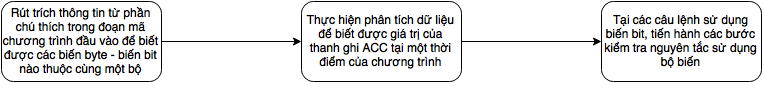
\includegraphics[width=0.7\linewidth]{image/soDoTypeChecking}
	\caption{Sơ đồ các bước thực hiện giải pháp Kiểm tra kiểu}
	\label{fig:sodotypechecking}
\end{figure}

Các phần tiếp theo của chương sẽ trình bày lần lượt các bước này.

\section{Chỉnh sửa để Boomerang chấp nhận việc sử dụng biến không phải thanh ghi}
\subsection{Cơ chế lưu trữ tên thanh ghi hiện nay của Boomerang}
Khi chuyển đổi từ mã assembly sang mã trung gian, Boomerang sẽ dùng một class con của Expr để biểu diễn thanh ghi. Cụ thể là class Location, và gọi phương thức static của class Location là Location::regOf(int num). Ta sẽ truyền vào phương thức này một con số đại diện cho thanh ghi đó. Cặp số - tên thanh ghi này được lưu vào một từ điển, để sau này khi thực hiện phân tích xong thì sẽ chuyển lại từ thanh ghi thành biến cục bộ.

Trong phần giải mã từ mã assembly sang mã trung gian, có một hàm để map giữa tên thanh ghi và con số đại diện cho nó, đó là hàm map\_sfr(string name).
\begin{lstlisting}[caption={Một số phần mã trong hàm map\_sfr},label={list:listmapsfr}]
if (name == "R0") return 0;
else if (name == "R1") return 1;
else if (name == "R2") return 2;
...
else return -1;

\end{lstlisting}

Sau khi trải qua các quá trình phân tích và đến giai đoạn in ra mã đầu ra, trình dịch ngược sẽ gọi hàm getRegName trong class FrontEnd để trả lại tên ban đầu của thanh ghi. Trong hàm getRegName sẽ lấy từ điển tên thanh ghi - số đại diện được quy định sẵn của mỗi phần giải mã cho các kiến trúc máy khác nhau, tìm tên thanh ghi tương ứng với con số đó và trả về.
\begin{lstlisting}[caption={Phần mã trong hàm getRegName},label={list:listgetregname}]
std::map<std::string, int, std::less<std::string> >::iterator it;
for (it = decoder->getRTLDict().RegMap.begin();	 it != decoder->getRTLDict().RegMap.end(); it++)
if ((*it).second == idx) 
return (*it).first.c_str();
return NULL;
\end{lstlisting}


Như vậy, có thể thấy với các tên biến không được quy định trước, hàm map\_sfr sẽ trả về giá trị -1, và vì giá trị -1 sẽ không có trong từ điển của phần giải mã, nên hàm getRegName sẽ trả về NULL, dẫn đến trình dịch ngược sẽ bị lỗi runtime và dừng ngay lập tức.\\

%lấy mã Boomerang ban đầu về, hiện kết quả khi sử dụng biến đầu vào

Vì số lượng tên biến là rất nhiều, nên ta không thể sử dụng phương pháp thêm mới các tên biến vào từ điển được quy định sẵn được, mà phải có cách để trình dịch ngược linh động hơn, chấp nhận bất kỳ các tên nào được sử dụng trong mã assembly. Giải pháp đưa ra là ngoài việc sử dụng từ điển thanh ghi được quy định sẵn, ta sẽ lập thêm một bảng tên biến, thành phần bao gồm các cặp tên biến - số đại diện. Trong giai đoạn giải mã, khi hàm map\_sfr được gọi, nếu tên truyền vào nằm trong các thanh ghi đã quy định sẵn, thay vì trả về giá trị -1 thì ta sẽ tạo ra một giá trị random và đưa chúng vào bảng tên biến ở trên. Ngoài ra, còn có một đoạn mã kiểm tra biến được sử dụng đã được khai báo bằng câu lệnh \#DEFINE chưa (ngoại trừ một số biến đặc biệt được tự sinh). \\
\begin{lstlisting}[caption={Phần mã mới được bổ sung trong hàm map\_sfr},label={list:listmapsfrnew},language=c++]
bool isDefined = false;
map<char*, AssemblyArgument*>::iterator it;
for (it = replacement.begin(); it!=replacement.end(); it++){
if(strcmp((*it).first, name.c_str()) == 0 ){
isDefined = true;
break;
}
}
if (isDefined || name.find("specbits") != string::npos ){
if (symbolTable->find(name) == symbolTable->end()){
bool existed = false;
int num;
do{
num = std::rand()%200+31;
map<string, int>::iterator it;
for (it = symbolTable->begin(); it!=symbolTable->end(); it++){
bool cond1 = (*it).second == num;
bool cond2 = (byteVar != -1 && byteVar>=num);
bool cond3 = (bit != -1 && bit>=num);
if (cond1 || cond2 || cond3){
existed = true;
continue;
} else {
existed = false;
}
}
} while (existed); 
(*symbolTable)[name] = num;
if (name.find("specbits") != string::npos){
std::cout<<"Name: "<<name<<", "<<num<<endl;
}
return num;
} else {
return symbolTable->find(name)->second;
}
}
else {
std::cout<<"ERROR: "<<name<<" HAS NOT BEEN DEFINED YET"<<endl;
exit(1);
}
\end{lstlisting}
Tương ứng với sự thay đổi ở hàm map\_sfr,  ở hàm getRegName, ngoài việc dò trong từ điển quy định trước, ta sẽ thêm một đoạn mã để dò trong bảng tên biến. 
\begin{lstlisting}[caption={Phần mã mới được bổ sung trong hàm getRegName},label={list:listgetregnamenew},language=c++]
std::map<string,int>::iterator symIt;
for (symIt = decoder->getSymbolTable().begin(); symIt != decoder->getSymbolTable().end(); symIt++){
	if ((*symIt).second == idx){
		return (*symIt).first.c_str();
	}
}
\end{lstlisting}
Như vậy, vấn đề giữ nguyên tên biến được giải quyết mà không ảnh hưởng nhiều tới trình dịch ngược.
%đoạn mã đầu vào assembly và mã đầu ra giữ nguyên được tên biến
\section{Mẫu khai báo biến byte và biến bit}
Sau khi đã thực hiện phần giữ nguyên tên biến, bước bắt buộc cho cả hai giải pháp, ta sẽ đi vào tìm hiểu bước đầu tiên của giải pháp Kiểm tra kiểu là đưa ra mẫu khai báo. Mẫu khai báo biến byte và biến bit được quy định như sau:
\begin{lstlisting}[caption={Mẫu khai báo bộ biến},label={list:listdeclarevar}]
;BEGIN DEFINE
;BYTE VAR
[byte var declare]
;BIT VAR
[eight bit var declares]
;END DEFINE
\end{lstlisting}
Đây là mẫu khai báo khi muốn gom các biến vào cùng một bộ, ngoài ra, chương trình vẫn chấp nhận việc khai báo riêng lẻ từng biến. Như vậy, cần chỉnh lại phần parser của trình dịch ngược để chấp nhận cấu trúc mới này. Ngoài ra, trong trình dịch ngược, cần có một cấu trúc mới để lưu trữ thông tin của các bộ biến byte và biến bit này. Trong đoạn mã \ref{list:listuniondefine}, có một trường byteVar để lưu tên biến byte, và một map lưu thứ tự của biến bit và tên biến bit tương ứng. Hiện tại, cấu trúc này đã đủ cho giải pháp Kiểm tra kiểu. Tuy nhiên, nó sẽ được mở rộng ở giải pháp sau. 
\begin{lstlisting}[caption={Cấu trúc dữ liệu để lưu trữ một bộ biến},label={list:listuniondefine}]
class UnionDefine{
	public:
	char* byteVar;
	map<int, char*>* bitVar;
	void prints(){
		cout << "Byte var: " << byteVar <<endl;
		cout << "Bit vars: "<<endl;
		map<int, char*>::iterator mi;
		for (mi = bitVar->begin(); mi != bitVar -> end(); mi++){
			cout << (*mi).second << ": " 
				<< (*mi).first << endl;
		}
	}
};
\end{lstlisting}
Như vậy, ta cần phải điều chỉnh lại phần parser của trình dịch ngược, sao cho nó vừa chấp nhận mẫu khai báo biến trên, vừa đưa từng bộ biến được khai báo vào trong một thực thể của class UnionDefine. Kết quả là, sau khi kết thúc phần parser, ta sẽ thu được một danh sách các class UnionDefine tương ứng với các khai báo ở trên. Đoạn mã \ref{list:listparser} là phần parser viết dựa trên thư viện Bison++ để thực hiện chức năng trên.\\
\begin{lstlisting}[caption={Đoạn mã parser cho phần khai báo bộ biến},label={list:listparser}]
definebit: BEGINDEFINE END\_LINE DEFINEBYTE END\_LINE define DEFINEBITS END\_LINE defineeachbit defineeachbit
defineeachbit defineeachbit defineeachbit defineeachbit defineeachbit defineeachbit ENDDEFINE END_LINE
{
	UnionDefine* ut = new UnionDefine();
	\$5 -> expList -> pop_back();
	ut->byteVar = \$5 -> expList -> back() -> argList.back()->value.c;
	ut->bitVar = bitVar;
	unionDefine1 -> push_back(ut);
	bitVar = new map<char\*, int>();
}
;
defineeachbit: DEFINE ID bit END_LINE {
	std::string temp(\$3->value.c);
	char c =  temp.at(temp.size()-1);
	int num = c - '0';
	(*bitVar)[\$2] = num;
}
;
\end{lstlisting}
Như vậy, sau giai đoạn parser, ta đã thu được bộ biến theo khai báo của người dùng. Tuy nhiên, nguyên tắc sử dụng bộ biến này là không bắt buộc trong quá trình lập trình 8051, và các assembler cũng không hề kiểm tra việc người dùng có tuân thủ nguyên tắc này không. Vì vậy, trước khi chuyển hoá các bộ biến này sang cấu trúc union ở mã đầu ra, ta cần phải kiểm tra đoạn mã của người dùng sử dụng các bộ biến như thế nào.

\section{Phân tích Reaching definitions}

Mục đích của phân tích Reaching definitions là biết được ở một thời điểm của chương trình, các câu lệnh khai báo nào đang còn hiệu lực, hay nói cách khác là gía trị của các biến đang được khai báo bởi những câu lệnh nào.
\begin{figure}
	\centering
	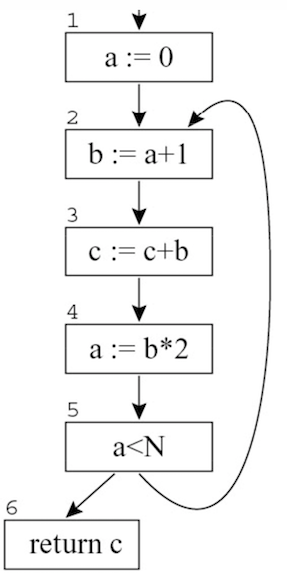
\includegraphics[scale=0.75]{image/reachingDefExam}
	\caption{Một đoạn chương trình mẫu}
	\label{fig:reachingdefexam}
\end{figure}
Ví dụ như ở đoạn chương trình \ref{fig:reachingdefexam}, ta cần biết được giá trị của biến a ở câu lệnh số 2 được khai báo ở câu lệnh này. Đối với con người thì rất dễ dàng biết được là biến a được sử dụng có thể khai báo ở câu lệnh số 1 hoặc câu lệnh số 5. Tuy nhiên, cần có một phương pháp phân tích để cho máy tính cũng biết được điều đó, và đó chính là phương pháp Reaching definitions. Như vậy, khi áp dụng vào trình dịch ngược, ta sẽ biết được tại thời điểm sử dụng biến bit, giá trị của thanh ghi ACC đang được định nghĩa ở câu lệnh nào. Từ đó tiến hành các bước kiểm tra tiếp theo. \\

Để thực hiện Reaching definitions, ta phải làm quen với các định nghĩa sau:
\begin{itemize}
	\item Nếu một biến được khai báo ở câu lệnh def1, sau đó được khai báo lại ở câu lệnh def2 sau đó, thì ta nói là câu lệnh def1 đã bị giết (killed) bởi câu lệnh def2.
	\item Nếu có một đường thực thi chương trình đi từ câu lệnh khai báo def1 đến một điểm p của chương trình, mà trên đó def1 không bị giết bởi bất kỳ câu lệnh nào, thì ta nói là def1 đã đến được điểm p. Khái niệm một câu lệnh đến được một basicblock cũng tương tự như vậy.
\end{itemize}

Ngoài ra, ta phải quy định một số khái niệm mới cho một basicblock B:
\begin{itemize}
	\item REACHin(B): Tập hợp các câu lệnh khai báo đến được đầu vào (entry) của B.
	\item REACHout(B): Tập hợp các câu lệnh khai báo đến được ngõ ra (exit) của B.
	\item GEN(B): Tập hợp các câu lệnh khai báo xuất hiện trong B và có thể đến được ngõ ra (exit) của B, nghĩa là biến được khai báo trong câu lệnh đó không được khai báo lại ở các câu lệnh đằng sau nó.
	\item KILL(B): Tập hợp các câu lệnh khai báo mà biến được khai báo đã được khai báo lại trong B.
\end{itemize}

Như vậy, mục tiêu của phân tích Reaching definitions ở cấp độ basicblock là tìm ra được tập hợp REACHin và REACHout của từng khối. Công thức được áp dụng là;
\begin{equation} \label{eq:reachout}
	REACHout(B) = GEN(B) \cup (REACHin(B)-KILL(B))
\end{equation}	
\begin{equation} \label{eq:reachin}
REACHin(B) = \cup_{j \in Pred(B)} REACHout(j)
\end{equation}	

Từ hai công thức \ref{eq:reachout} và \ref{eq:reachin}, ta thấy ở phân tích này, tập hợp các giá trị ra (REACHin) được quyết định bởi các giá trị vào (REACHout), ngược lại với phân tích liveness. Như vậy, luồng đi của phân tích là xuôi với luồng đi của chương trình. Theo mẫu thường thấp của một phân tích dữ liệu, ta sẽ lần lượt tính toán các tập hợp vào và tập hợp ra của từng basicblock cho đến khi không còn thay đổi nào được ghi nhận. Xem sơ đồ khối bên dưới.

\begin{figure}
	\centering
	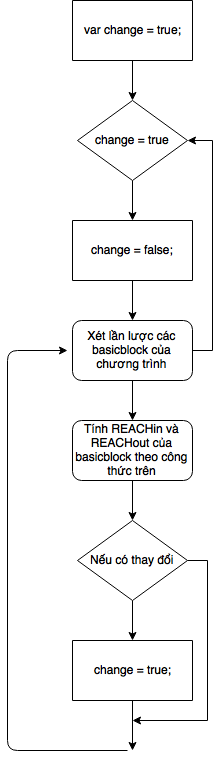
\includegraphics[scale=0.75]{image/reachingDefAlgo}
	\caption{Giải thuật tính Reaching definitions cho basicblock}
	\label{fig:reachingdefalgo}
\end{figure}

Tuy nhiên, trong trường hợp của bài toán cần giải quyết, ta cần phải biết tập hợp ra vào của từng câu lệnh một, chứ không chỉ của toàn bộ basicblock, vì vậy, khi ứng dụng vào Boomerang, giải thuật sẽ được điều chỉnh lại để tìm tập REACHin và REACHout của từng câu lệnh. Việc điều chỉnh này là khá nhỏ, và các bước vẫn sẽ giữ nguyên, không thay đổi nhiều.\\

Tuy nhiên, phân tích Reaching definitions chỉ cho biết được câu lệnh khai báo có hiệu lực của một biến tại một thời điểm chương trình, chứ không cho biết được giá trị thực sự của biến đó. Nếu vế phải của câu lệnh khai báo này chỉ đơn giản là pointer của một biến byte, thì ta sẽ dễ dàng kiểm tra được. Nhưng ngoài ra, biểu thức nằm trong dấu pointer khi dịch ngược từ mã assembly 8051 lên có thể là các trường hợp sau đây:
\begin{itemize}
	\item Một hằng số.
		\item Một thanh ghi, giá trị của thanh ghi có thể được khai báo ở các câu lệnh trước đó.
	\item Một biểu thức có hai vế, các vế của biểu thức có thể là một biến, một thanh ghi hoặc một hằng số.

\end{itemize}

\begin{lstlisting}[caption={Một số câu lệnh gán mà phương pháp Suy luận kiểu sử dụng Reaching definitions không xử lý được},label={list:listhardcase}]
MOV A, 38H
MOV A, @DPTR
MOV A, OPTION+1
\end{lstlisting}
Với phương pháp Reaching definitions, ta sẽ không thể xử lý được với các trường hợp phức tạp hơn như các câu lệnh trong đoạn mã \ref{list:listhardcase}. Ta sẽ không biết được biến byte nào đã được khai báo giá trị 38H, hoặc thanh ghi DPTR đã được gán giá trị gì trước đó, hoặc OPTION+1 có bằng giá trị của một biến byte nào khác không... Ngoài ra, với trường hợp trong tập hợp REACHin của câu lệnh có nhiều câu lệnh khai báo cho thanh ghi ACC, ta sẽ không thể kiểm tra được vế phải của tất cả các câu lệnh khai báo đó có cùng một giá trị hay không mà chỉ đơn giản xử lý là câu lệnh đã vi phạm nguyên tắc sử dụng bộ biến. Như vậy sẽ làm giảm độ chính xác trong quá trình tìm các bộ biến. Một phân tích khác sẽ được áp dụng trong giai đoạn tiến hành giải pháp Suy luận kiểu. Còn với giai đoạn sơ khai này của luận văn, ta sẽ giả thuyết rằng ở đoạn mã đầu vào chỉ có các câu lệnh gán vùng nhớ đơn giản cho ACC với một biến byte duy nhất như đoạn mã \ref{list:listeasycase}.
\begin{lstlisting}[caption={Mẫu câu lệnh gán cho thanh ghi ACC được chấp nhận hiện giờ},label={list:listeasycase}]
MOV A, OPTIONS
\end{lstlisting}
\section{Kiểm tra cách sử dụng bộ biến trong toàn bộ chương trình và sinh mã}

\label{sec:laststep}
Sau khi đã có thông tin về tập hợp các câu lệnh khai báo có hiệu lực ở tất cả các câu lệnh của chương trình, ta sẽ chuyển sang kiểm tra các ở các câu lệnh sử dụng bit.

Quá trình kiểm tra cho 1 câu lệnh sử dụng bit gồm các bước sau:

\begin{figure}
	\centering
	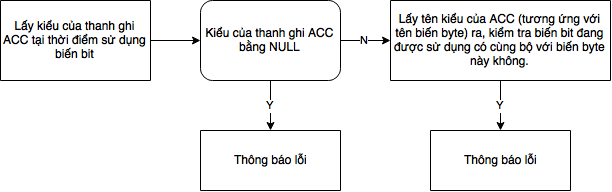
\includegraphics[width=0.7\linewidth]{image/checkUnionSteps}
	\caption{Quá trình kiểm tra một câu lệnh sử dụng bit}
	\label{fig:checkunionsteps}
\end{figure}

Nếu ở bất cứ câu lệnh sử dụng biến bit nào, nguyên tắc đưa ra bị vi phạm, thì trình dịch ngược sẽ hiện thông báo lỗi trên console cho người dùng. Sau đó, đoạn mã kiểm tra lỗi vẫn tiếp tục chạy để kiểm tra các câu lệnh khác nhằm tạo thuận lợi cho người dùng trong quá trình sửa lỗi chương trình đầu vào. Tuy nhiên, nếu có lỗi thì trình dịch ngược sẽ không sinh mã đầu ra vì sẽ không thể xử lý được sinh các union như thế nào.

%đoạn mã và output của trình dịch ngược khi vi phạm nguyên tắc sử dụng

Kết thúc quá trình kiểm tra lỗi, nếu không có vi phạm nào xảy ra, trình dịch ngược sẽ tiến hành sinh ra thêm một số khai báo cho bộ biến, cũng như thực hiện các thay thế cần thiết. Các bộ biến được khai báo được lưu bằng cấu trúc UnionDefine, và ta cần thể hiện các bộ biến đó bằng một cấu trúc dữ liệu ở ngôn ngữ cấp cao của mã đầu ra. Như đã phân tích từ trước ở chương \ref{sec:gioithieu}, cấu trúc dữ liệu đó là union. Hình \ref{fig:uniondefinemapping} thể hiện việc chuyển đổi của class UnionDefine sang cấu trúc union.

\begin{figure}
	\centering
	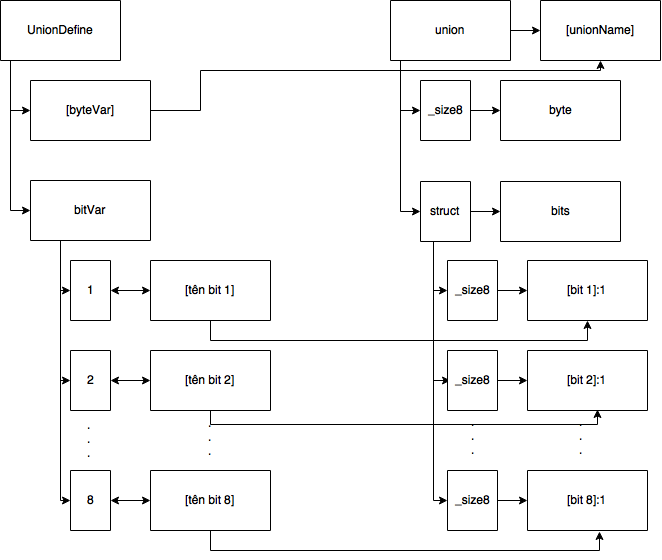
\includegraphics[width=0.7\linewidth]{image/unionDefineMapping}
	\caption{Hình minh hoạ việc chuyển đổi từ class UnionDefine sang cấu trúc union ở mã đầu ra}
	\label{fig:uniondefinemapping}
\end{figure}

Sau khi sinh ra các union như trên, ta cần tiến hành thực hiện các thay thế sau:
\begin{itemize}
	\item Thay thế các biểu thức thể hiện biến bit dưới dạng thanh ghi độc lập thành một biểu thức truy xuất đến một thành phần của union tương ứng với bộ biến mà biến bit đó thuộc về. Vì ở giai đoạn giải mã, ta không thực hiện kiểm tra biến nào là biến bit, biến nào là biến byte, nên ta sẽ xem tất cả các biến như những thanh ghi độc lập nhau. Sau khi đã trải qua các quá trình phân tích và sinh ra các union, ta cần thay thế để thể hiện rõ mối liên hệ giữa biến bit và biến byte.
	
	\item Thay thế các biểu thức truy xuất trực tiếp bit của thanh ghi ACC thành biểu thức truy xuất đến một thành phần của union tương ứng với bộ biến chứa biến byte mà thanh ghi ACC đang mang giá trị trỏ đến. Vì một số lý do, có đôi khi người lập trình viên không sử dụng biến bit mà sử dụng một truy xuất trực tiếp đến bit trong thanh ghi ACC, ví dụ như: ACC.1. Với trường hợp này, vì ta đã có trong tay bộ biến và giá trị của biến byte thanh ghi ACC đang được trỏ đến, ta sẽ thay thế để đoạn mã đầu ra thống nhất hơn, và có thể tiến hành bước thay thế thanh ghi ACC được trình bày bên dưới. Lưu ý: trong giai đoạn giải mã, ghi gặp biểu thức ACC.x, trình giải mã sẽ chuyển chúng về một thanh ghi đặc biệt có tên là specbitsx, với x là số thứ tự của bit muốn truy xuất (xem ví dụ đoạn mã \ref{list:listbeforereplacebit}).
	\begin{lstlisting}[caption={Mã đầu ra trước khi thực hiện bước thay thế biến bit},label={list:listbeforereplacebit}, language = c]
	TESTSUPS = 1;
	if (specbits5 == 1){
		 ...
	}
	\end{lstlisting}
	
	\begin{lstlisting}[caption={Mã đầu ra sau khi thực hiện bước thay thế biến bit},label={list:listafterreplacebit}, language = c]
	OPTIONS.bits.TESTSUPS = 1;
	if (OPTIONS.bits.bit1 == 1){
		...
	}
	\end{lstlisting}
\begin{lstlisting}[caption={Mã đầu ra trước khi thực hiện bước thay thế thanh ghi ACC},label={list:listbeforereplace}]
a = *OPTIONS;
OPTIONS.bits.TESTSUPS1 = 1;
return a;
\end{lstlisting}
\begin{lstlisting}[caption={Mã đầu ra sau khi thực hiện bước thay thế thanh ghi ACC},label={list:listafterreplace}]
OPTIONS.bits.TESTUPS1 = 1;
return OPTIONS.byte;
\end{lstlisting}
\item Thay thế các vị trí sử dụng thanh ghi ACC bằng biến byte tương ứng. Khi lập trình ở dạng mã assembly, lập trình viên không được phép xử lý các vùng nhớ trực tiếp mà phải thông qua thanh ghi, tuy nhiên, khi đã chuyển đổi về dạng ngôn ngữ cấp cao, ta có thể sử dụng trực tiếp tên biến trong các câu lệnh mà không cần trung gian qua thanh ghi nữa. Điều này giúp mã đầu ra dễ hiểu và trong sáng hơn.

\begin{lstlisting}[caption={Mã đầu ra trước khi thực hiện bước thay thế thanh ghi ACC},label={list:listbeforereplace}]
a = *OPTIONS;
OPTIONS.bits.TESTSUPS1 = 1;
return a;
\end{lstlisting}
\begin{lstlisting}[caption={Mã đầu ra sau khi thực hiện bước thay thế thanh ghi ACC},label={list:listafterreplace}]
OPTIONS.bits.TESTUPS1 = 1;
return OPTIONS.byte;
\end{lstlisting}
\end{itemize}


Như vậy, với giải pháp Kiểm tra kiểu này, ta đã có sẵn thông tin về bộ biến ngay từ đầu và chỉ cần kiểm tra xem người lập trình có tuân thủ đúng quy tắc không trước khi sinh ra mã ở ngôn ngữ cấp cao. Giải pháp này yêu cầu can thiệp vào trình dịch ngược ít và hiện thực dễ dàng. Tuy nhiên, giải pháp còn nhiều hạn chế như phương pháp phân tích dữ liệu chưa đạt độ chính xác cao, cần người dùng phải chỉnh sửa lại khai báo theo mẫu quy định... Chính vì vậy, giai đoạn sau của luận văn đã phát triển một giải pháp mới có độ chính xác cao hơn và không cần chỉnh sửa mã đầu vào của người dùng, đó là giải pháp Suy luận kiểu. Giải pháp này sẽ được trình bày ở chương tiếp theo.



